\section{Codes to Improve Accesses}
\label{sec:code_design}

%In this section, we discuss one of the main components of the memory design proposed in this paper. 
As a key idea behind the memory designs proposed in this paper, we plan to utilize coding schemes to introduce the redundancy into the storage space comprising an array of single-port memory banks in order to support multiple accesses to the array. For this approach to be successful, it's important to work with the right coding schemes which are designed by keeping the access-efficiency as the central criterion. In this section, we describe three such coding schemes that we employ for the task of emulation of multi-port memories using single-port memory banks. Before presenting these coding schemes, we first introduce some basic concepts and terminology that we use throughout the rest of this paper.

\begin{comment}
Coding theory is the study of codes and their applications  to specific fields.  
Coding has been used in a variety of computer  science applications,  from error 
correction in the transmission of data  to increased compression for data  
storage.  We aim to extend the benefits of coding theory  to improve the 
efficiency of random-access  memory systems.  We propose a memory scheme in 
which a small portion of memory is reserved for the efficient coding of 
pre-existing data.  In essence, this allows the data of one bank to be 
duplicated and stored in an additional memory location.  Traditionally, when 
multiple  requests  to a single bank  are issued by the processor, a stall is 
generated.  These types of stalls, known as bank conflicts, result from the fact 
that  only one address from a single bank can be accessed at a time.  The 
processor must wait for the result from the first bank access to return  before 
it can serve additional  requests to the same bank.  This lag can be a major 
bottleneck in a computer's processing speed. With a coded memory scheme, data 
present in multiple data banks will be compressed and stored in extra banks, 
known as a parity banks.  These parity banks will then be accessed concurrently 
with corresponding data  banks to help alleviate stalls from bank conflicts.  
Ultimately,  with the addition  of a single parity  bank we are able to generate 
a single additional  access to any arbitrary bank  without  implementing  any 
further  logic to the bank  itself.  In the following sections, we first 
describe the design parameters used to design the coding system.  We then 
describe each of the three code designs explored in this project.
\end{comment}

\subsection{Coding for memory banks}
\label{sec:coding_mb}

A coding scheme is defined by its encoding process which maps a given collection of information elements to a larger and redundant collection of elements known as codeword. In the context of memory banks, we begin with {\em data banks} which refer to the memory bank storing the original information. The encoding process of the underlying coding scheme then utilize the content of these data banks to generate elements to be stored in the additional memory banks such the overall array of memory banks stores the information in a redundant manner. The additional memory banks are termed as {\em parity banks}. The encoding operations used to generate parity elements in this paper can be classified into two categories.
\begin{enumerate}
\item \textbf{Inter-bank encoding:~}A parity element depends on at most one element for each of the data banks.
\item \textbf{Intra-bank encoding:~}A parity element is generated using multiple elements from a data bank.
\end{enumerate}
Furthermore, we restrict ourselves to linear coding schemes which perform only linear operations (over a finite field) during the encoding process. In fact, in order to keep the computation complexity small, we only consider coding schemes over the binary field. This implies that the linear operations are nothing but $XOR$ operations. %This is equivalent to saying that the elements stored on the parity banks are linear functions of the elements stored on the data banks. 
The following example further clarifies these concepts along with some necessary notation with help of a coding scheme that employs only {inter-bank} encoding. 
\begin{example}
Let's consider a setup with two data banks $\mathbf{a}$ and $\mathbf{b}$. We assume that each of banks store $LW$ binary data elements\footnote{It is possible to work with data elements over larger alphabets/finite fields. However, assuming data elements to be binary suffices for us as we only work with coding schemes defined over binary field in this paper.} which are arranges in an $L \times W$ array. In particular, for $i \in [L] \triangleq \{1,\ldots, L\}$, $a(i)$ and $b(i)$ denote the $i$-th row of the bank $a$ and bank $\mathbf{b}$, respectively. Moreover, for $i \in [L]$ and $j \in [W] \triangleq \{1,\ldots, W\}$, we use $a_{i, j}$ and $b_{i, j}$ to denote the $j$-th element in the rows $a(i)$ and $b(i)$, respectively. Therefore, for $i \in [L]$, we have 
\begin{align}
a(i) = \big(a_{i,1}, a_{i,2},\ldots, a_{i, W}\big) \in \{0, 1\}^W\nonumber \\
b(i) = \big(b_{i,1}, b_{i,2},\ldots, b_{i, W}\big) \in \{0, 1\}^W. \nonumber
\end{align}
Now, consider a linear coding scheme that produces a parity bank $\mathbf{p}$ with $L'W$ bits arranged in an $L' \times W$ array such that for $i \in [L'] \triangleq \{1,\ldots, L'\}$, 
\begin{align}
p(i) &= \big(p_{i, 1},\ldots, p_{i,W}\big) \nonumber \\
&= a(i) + b(i) \nonumber \\
&\triangleq \big(a_{i,1}\oplus b_{i,1}, a_{i,1}\oplus b_{i,1},\ldots, a_{i,1}\oplus b_{i,1}\big). 
\end{align}
Figure~\ref{fig:example1_case1} illustrates this coding scheme. Since the parity bank is based on those rows of the data banks that are indexed by the set $[L'] \subseteq [L]$, we also use the following concise notation to represent the encoding of the parity bank. 
$$
\mathbf{p} = \mathbf{a}([L']) +  \mathbf{b}([L']).
$$
In general, we can use any subset $\mathcal{S} = \{i_1, i_2,\ldots, i_{L'}\} \subseteq [L]$ comprising $L'$ rows of data banks to generate the parity bank $\mathbf{p}$. In this case, we have
$$
\mathbf{p} = \mathbf{a}(\mathcal{S}) +  \mathbf{b}(\mathcal{S}),
$$ 
or
$$
p(l) = a(i_l) + b(i_l)~\text{for}~l \in [L'].
$$
Figure~\ref{fig:example1_case2} illustrates the case with $\mathcal{S} = [L - L'  + 1,\ldots, L]$.
\end{example}

%%%%%%%%%%%%%%%%%%%%%%%%%%%%%%%%%%%
\begin{figure}[t!]
\centering
\begin{subfigure}[b]{0.4\linewidth}
  \centering
  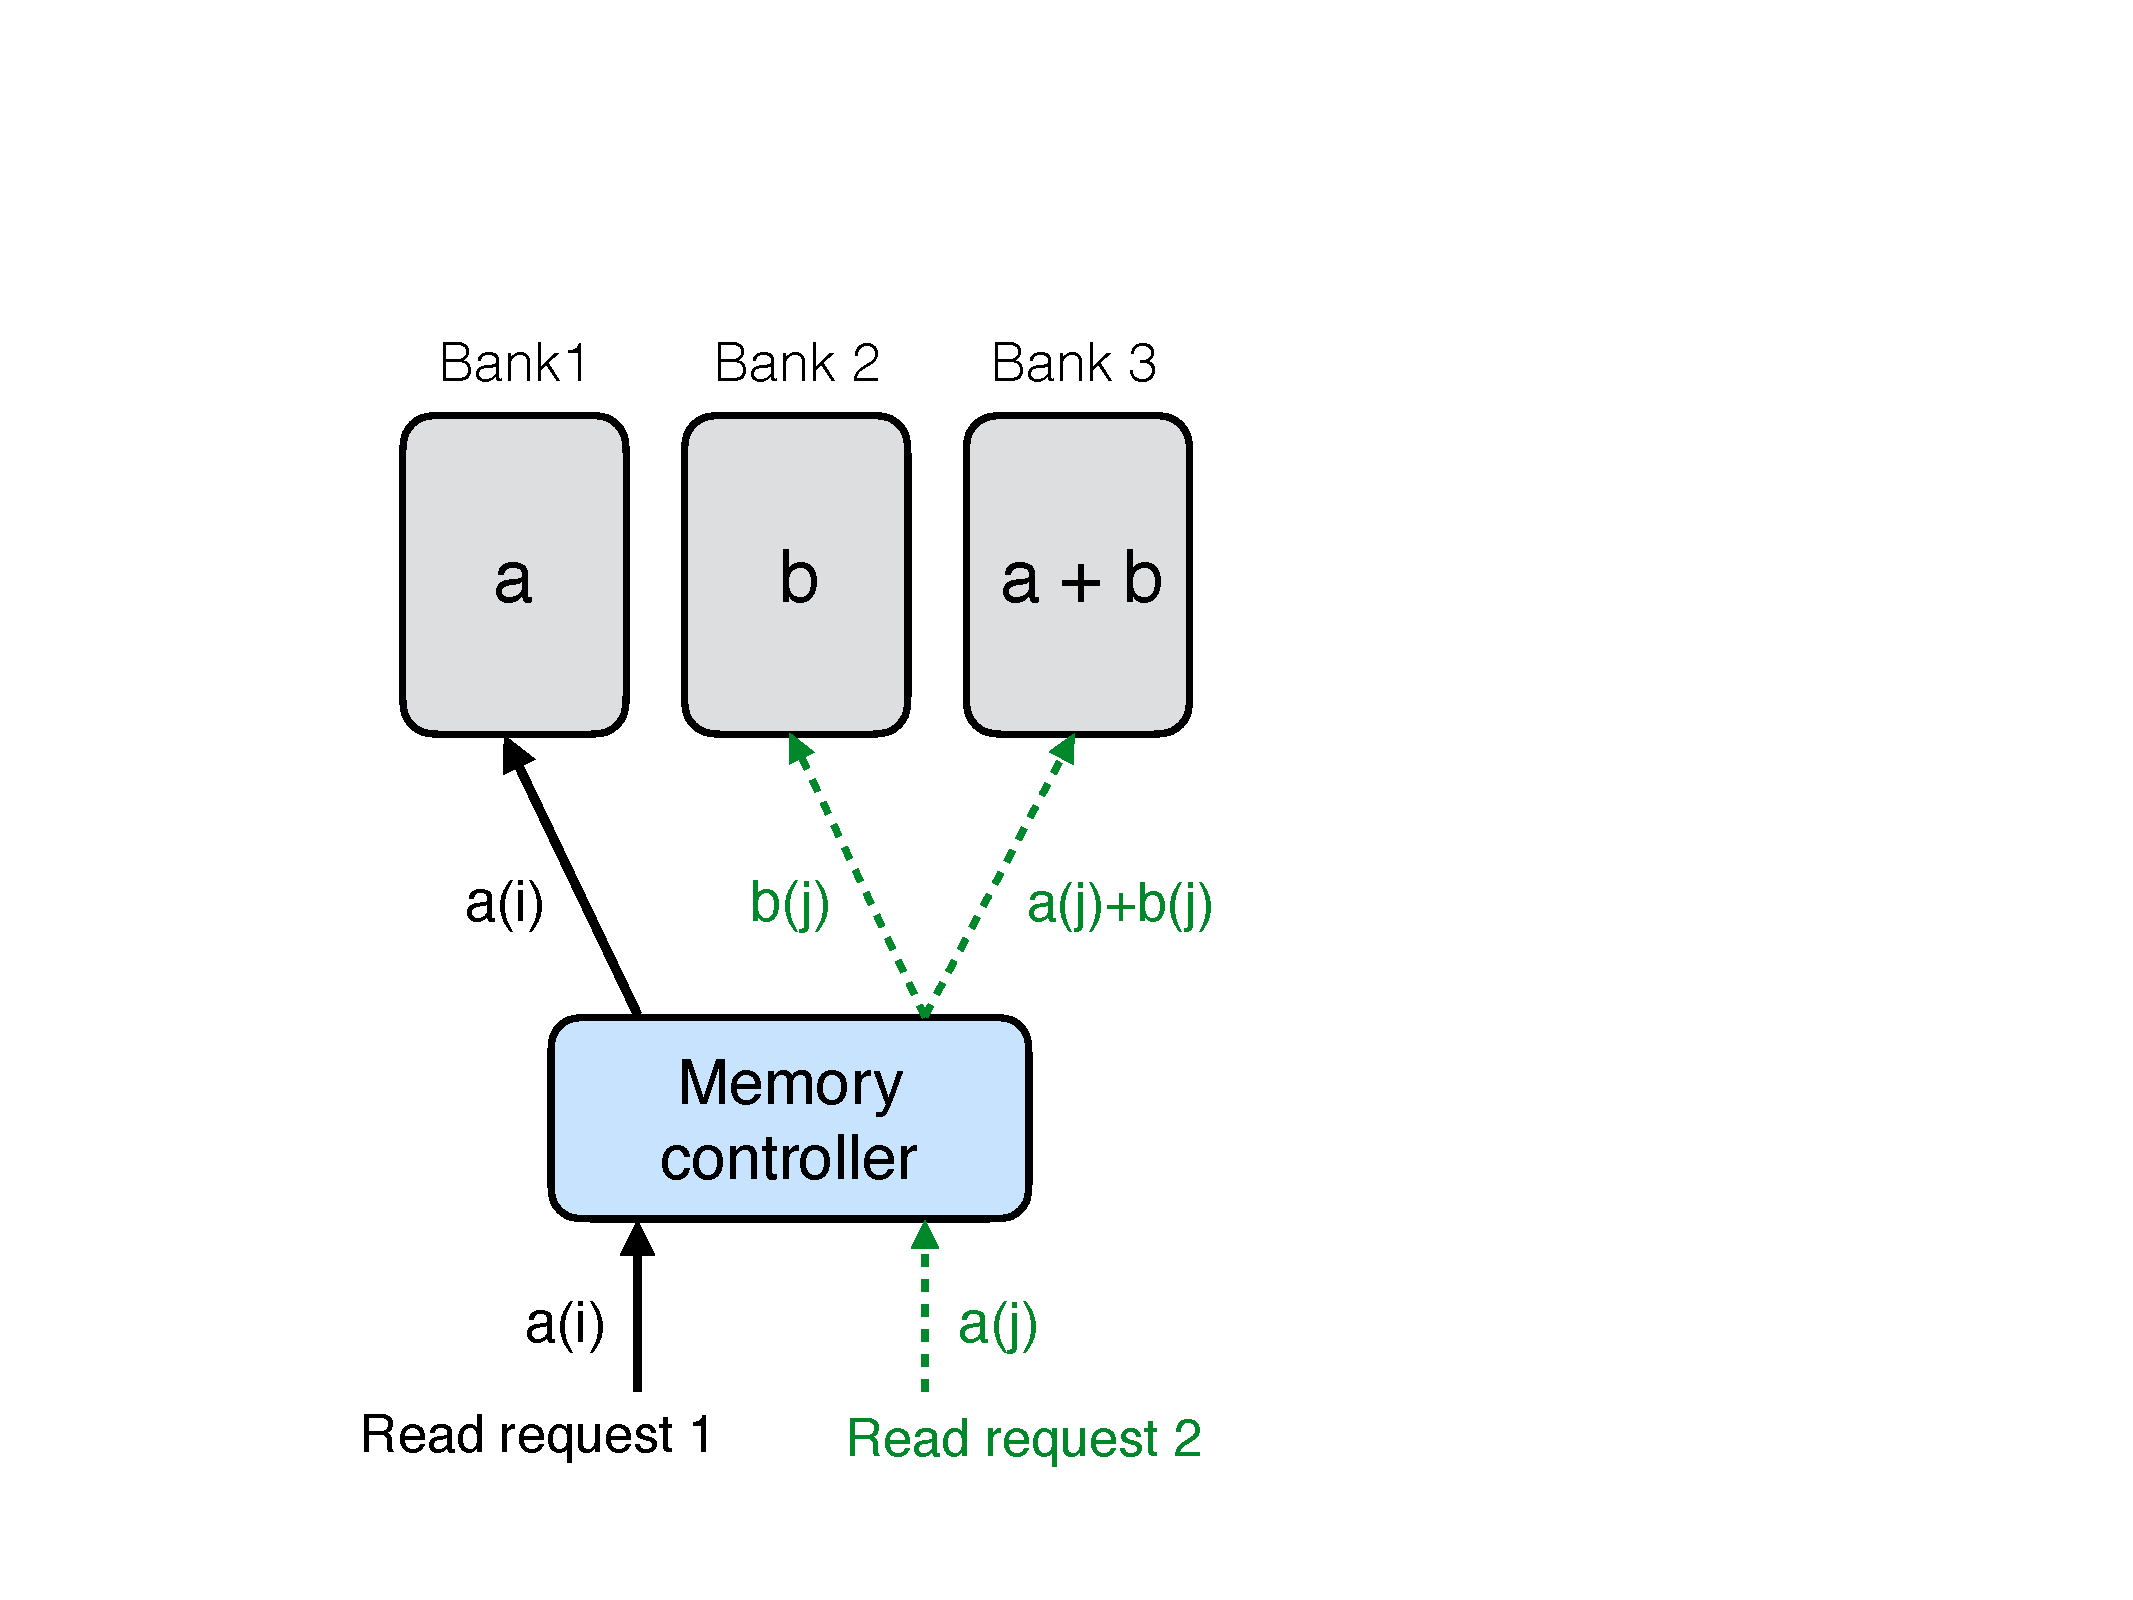
\includegraphics[width=0.9\linewidth]{fig/example-xor.pdf} 
  \caption{{\color{red}Parity.}}
  \label{fig:example1_case1}
\end{subfigure}
\begin{subfigure}[b]{0.4\linewidth}
  \centering
  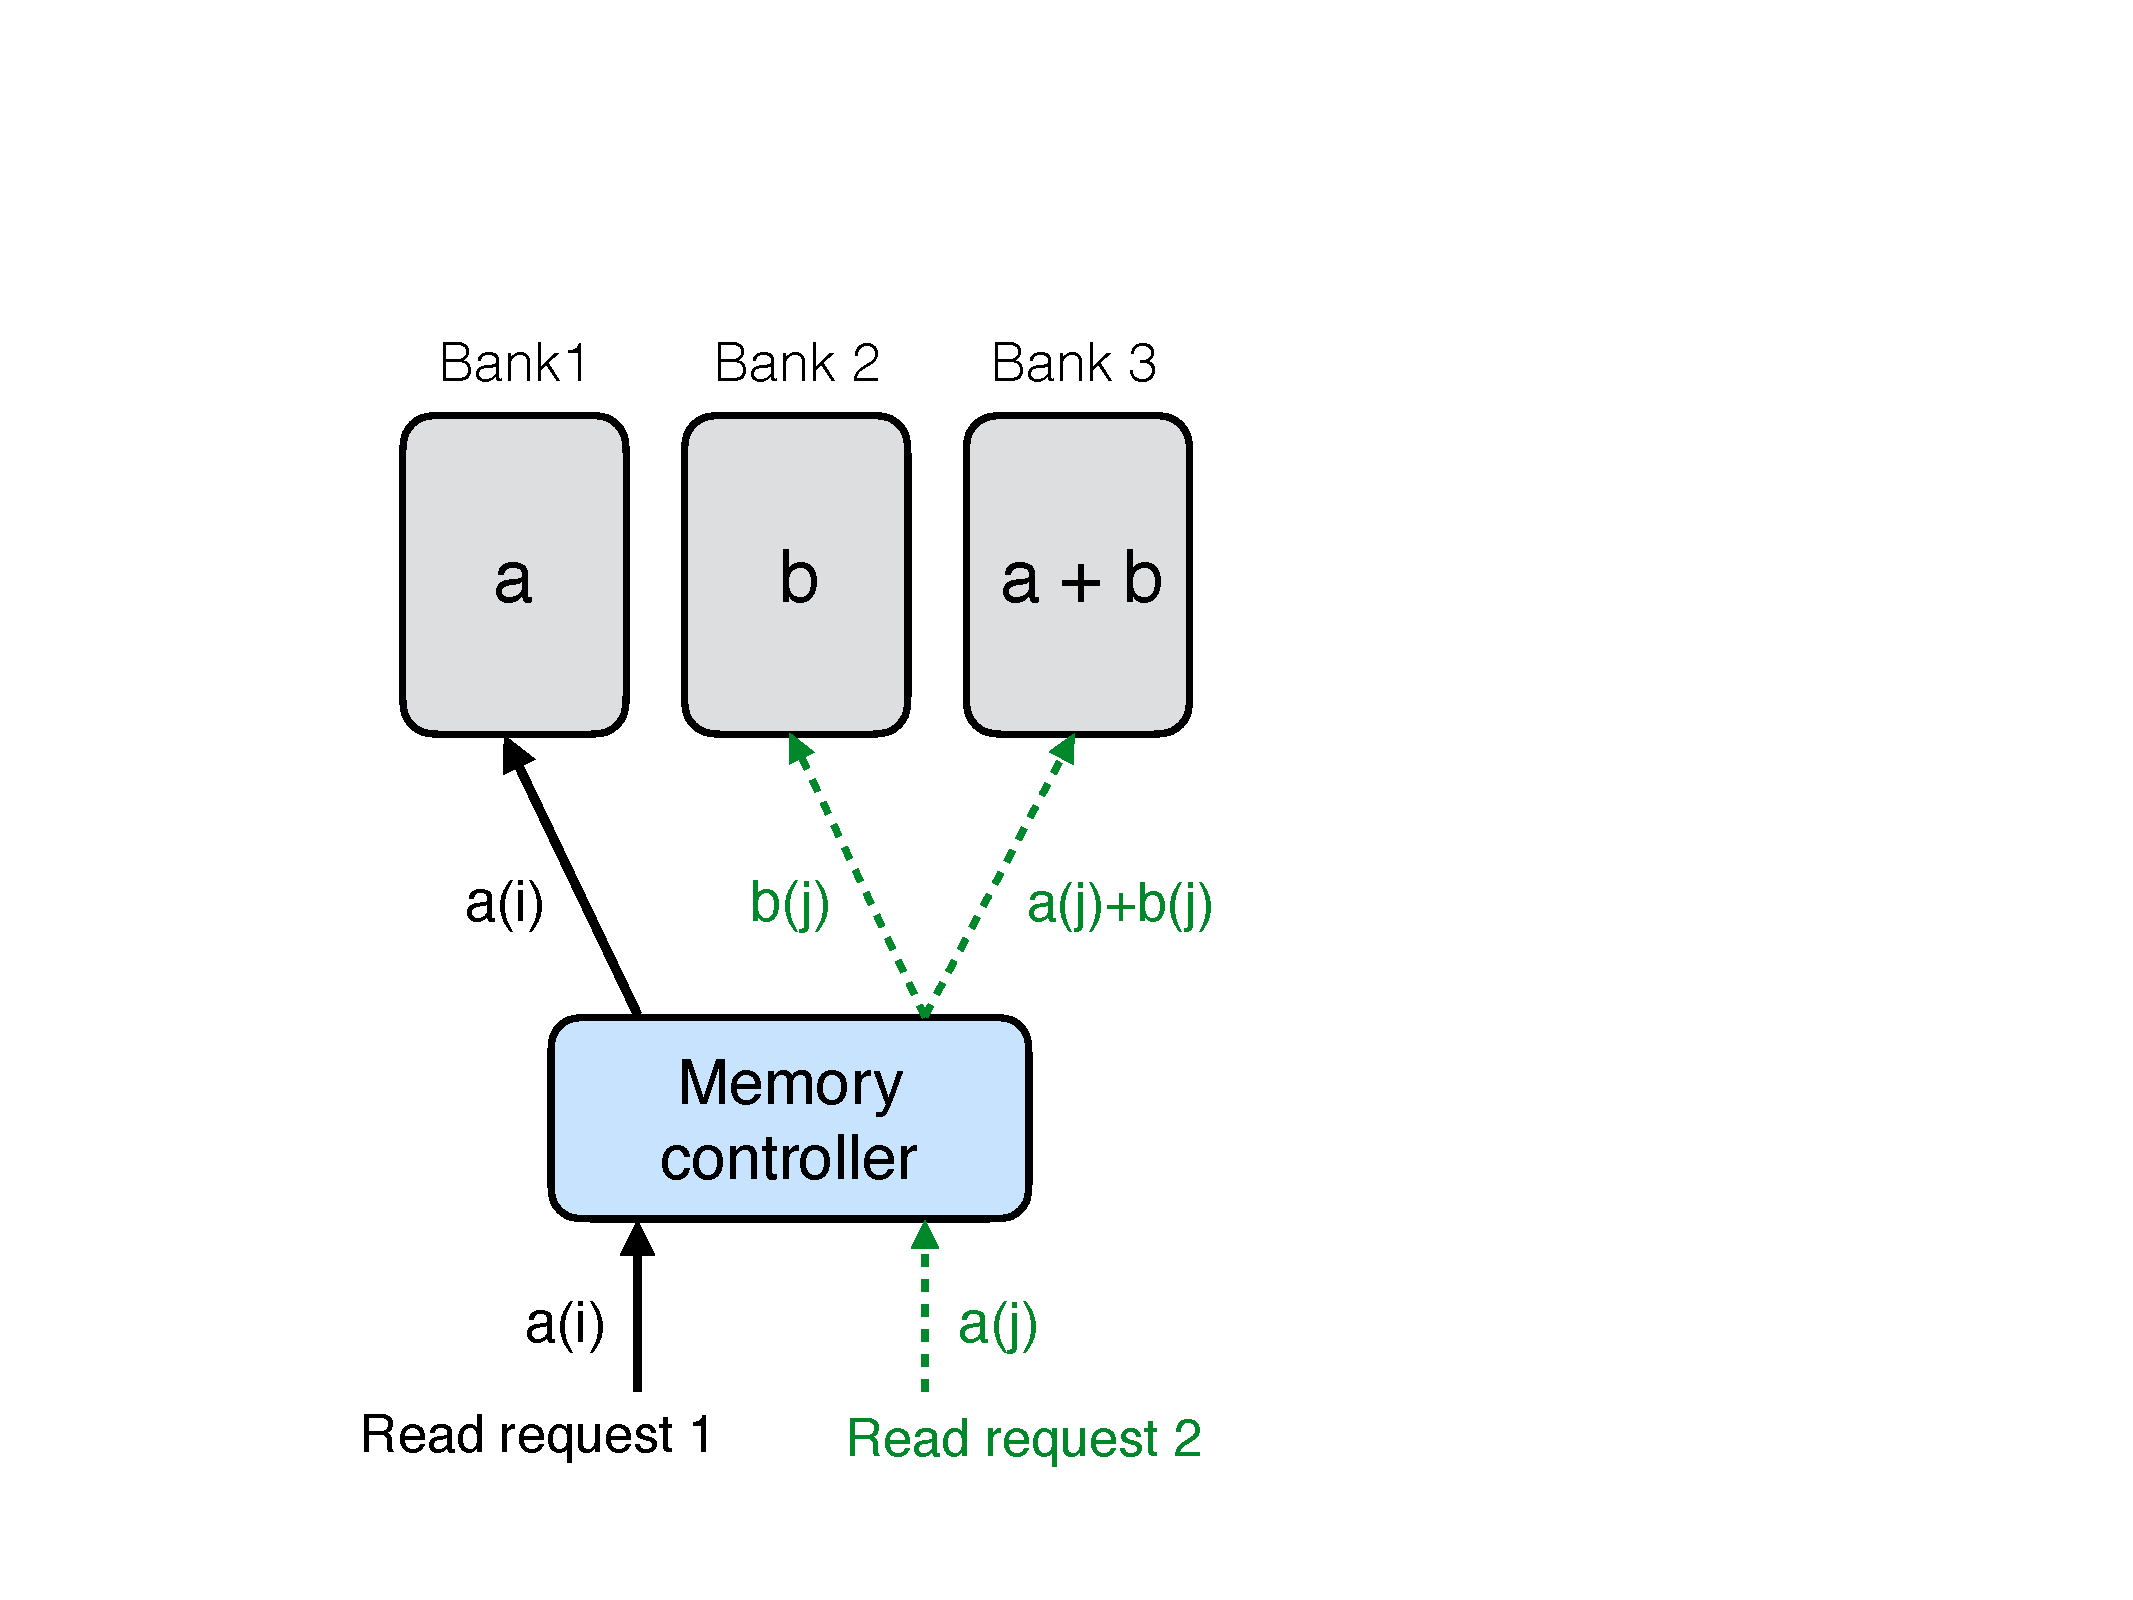
\includegraphics[width=0.9\linewidth]{fig/example-xor.pdf} 
  \caption{{\color{red}Parity.}}
  \label{fig:example1_case2}
\end{subfigure}
\caption{Design.}
\label{fig:example1}
\end{figure}
%%%%%%%%%%%%%%%%%%%%%%%%%%%%%%%%%%%%%%


\begin{remark}
{\color{red} Note that we allow for the data banks and parity banks to have different sizes, i.e., $L \neq L'$. This freedom in memory design can be utilized to reduce the storage overhead of parity banks based on the underlying application. The case when the size of a parity bank is smaller than a data bank, i.e., $L' < L$, we say that the parity bank is a {\em shallow bank}. We note that it's perfectly reasonable to have the provisions for shallow banks, especially in proprietary designs of integrated memories in a system on a chip (SoC).}
\end{remark}

\subsubsection{Degraded reads and their locality}
\label{sec:degraded}

Now let's focus on the application of redundant (encoded) data stored on an array of banks to improves the accesses to the original data elements by avoiding bank conflicts. Let's consider the coding scheme illustrated in Figure~\ref{fig:example1_case1}, where the parity bank $\mathbf{p} = \mathbf{a}([L']) + \mathbf{b}([L'])$. Now, given two read requests $\{a(1), a(L)\}$, which would have led to a bank conflict (at the data bank $\mathbf{a}$) without the parity banks, can now be simultaneously served without any bank conflicts: 1) Serve the request $a(L)$ from the data bank $\mathbf{a}$, and 2) Download $b(1)$ and $p(1) = a(1) + b(1)$ from the data bank $\mathbf{b}$ and the parity bank to serve $a(1)$ by reconstructing $a(1) = b(1) + p(1)$. A read request which is served with the help of parity banks (the request for $a(1)$ in this case) is termed as {\em degraded read}. Each degraded read has a parameter {\em locality} associated with it which corresponds to the total number of banks that need to be accessed to serve the degraded read. In this aforementioned case, the locality of the degraded read for $a(1)$ is $2$ as we access two banks, the data bank $\mathbf{b}$ and the parity bank $\mathbf{p}$, to perform the degraded read. 

In order to further illustrate the notion of locality, let's consider a setup where we generate a parity bank $\mathbf{p}$ by combining three data banks $\mathbf{a}$, $\mathbf{b}$, and $\mathbf{c}$ as $\mathbf{p} = \mathbf{a} + \mathbf{b} + \mathbf{c}$. Now, a degraded read for $a(1)$ using the parity bank as $$a(1) = b(1) + c(1) + p(1) = b(1) + c(1) + \big(a(1) + b(1) + c(1)\big)$$
has locality $3$ as the degraded read is served using three memory banks.

\subsection{Codes to emulate multi-port memory}
\label{sec:designs}

We are now in position to describe the code designs employed in this work to carry out the emulation of multi-port memories. Among a large set of possible coding schemes, we focus on three specific coding schemes  for this task. We believe that these three coding schemes strike a good balance among various quantities of interests, including storage overhead, number of simultaneous read requests supported by the array of banks, and the locality associated with various degraded reads. Furthermore, these coding schemes respect the practical constraint of encoding across a small number of data banks. In particular, we focus on the setup with $8$ memory banks. This is in contrast with the application of coding in communications, where encoding is performed over a much larger number of information symbols. 

In the rest of this section, we present the three code designs and discuss the number of simultaneous read requests supported by these designs both in the worst and the best case. We also summarize all the relevant parameters associated with these designs in Table~\ref{table:codedesigncomparison} which highlights the trade-offs among these parameters. 
%
%We discuss the design of the codes for creating extra accesses to memory in this 
%section. First we discuss the code designs explored during Phase I. Second, we discuss 
%specific execution strategies to efficiently implement the designs.\\
%In the following sub-sections, we discuss 3 designs for storing coded data.  
%Table~\ref{table:codedesigncomparison} compares these designs for various 
%parameters and associated costs.  
%\begin{table*}[t]
%\centering
%	\begin{tabular}{|m{1cm}|m{2 cm}|m{1cm}|m{1cm}|m{1cm}|m{1cm}|m{1cm}|}
%\hline
%Design & Max Read per bank & Max Write per bank & Locality & Rate & Memory 
%Overhead & Logical Complexity \\ \hline
%I & 4 & 2 & 2 & $2/5$ & 1.5 $\alpha$ & Low \\ \hline
%II & 5 & 2 & 2 & $2/5$ & 2.5 $\alpha$ & Medium \\ \hline
%III & 4 & 2 & 3 & $1/2$ & \text{      } $\alpha$ & Medium \\ \hline
%	\end{tabular}
%	\caption{Comparison of design with respect to the performance parameters 
%	and associated cost}
%	\label{table:codedesigncomparison}
%\end{table*}


\begin{scriptsize}
\begin{table*}[t!]
  \centering
  \begin{tabular}{|c|c|c|c|c|c|c|}
    \hline
    \textbf{Design} & \textbf{Max reads} & \textbf{Max writes} & \textbf{Locality} & \textbf{Rate} & \textbf{Storage overhead} & \textbf{Logical complexity} \\
    & \textbf{(per bank)} & \textbf{(per bank)} & & & & \\
    \hline
    \hline
    I & 4 & 2 & 2 & $2/5$ & 1.5 $\alpha$ & Low \\ \hline
II & 5 & 2 & 2 & $2/5$ & 2.5 $\alpha$ & Medium \\ \hline
III & 4 & 2 & 3 & $1/2$ & \text{      } $\alpha$ & Medium \\ 
\hline                                   
  \end{tabular}
	\caption{Comparison of the code designs with respect to the performance parameters and associated cost}
	\label{table:codedesigncomparison}
\end{table*}
\end{scriptsize}


\subsubsection{Code design I}
\label{sec:design1}

This code design is motivated from the concept of batch codes~\cite{batchcodes} which enables parallel access to the content stored in a large scale distributed storage system.  This design employs only inter-bank encoding across rows of data banks. The coding scheme is illustrated in Figure~\ref{fig:design1}. The code design involves $8$ data banks $\{\mathbf{a}, \mathbf{b},\ldots, \mathbf{h}\}$ (each of size $L$) and $12$ shallow banks (each of size $L' = \alpha L$ for $0< \alpha \leq 1$). We partition the $8$ data banks into two disjoint groups consisting of $4$ banks each. The underlying coding scheme produces (shallow) parity banks by separately encoding data banks from the two groups. Thus, as shown in Figure~\ref{fig:design1}, the entire array of banks, including data banks and parity banks, can be viewed as partitioned into two disjoint code region. For a specific choice of $\alpha$, the storage overhead of this design is $12\alpha L$ which amounts to the rate of the coding scheme being $$\frac{8L}{8L + 12\alpha L} = \frac{2}{2 + 3\alpha}.$$

\begin{remark}
\label{rem:design1}
Note that the size of shallow banks is a design choice which is controlled by the parameter $0 < \alpha \leq 1$. A small value of $\alpha$ corresponds to small storage overhead. However, $\alpha < 1$ ensures multiple access for only a subset of data elements (belonging to the encoded rows) from the data banks. The identity of the $L' = \alpha L$ rows from data banks that are encoded using the shallow parity banks depend on nature of access request being served by the memory system. In particular, in Section~\ref{sec:dynamicCoding} we discuss a dynamic coding approach that dynamically change the encoded rows based on the detection of the regions of memory banks that receive a large number of access requests. For applications, where such sustained concentration of access patterns is not present, one can employ design with $\alpha = 1$, i.e., the parity banks have the same size as the data banks and all the elements of the data banks are stored in the encoded form in the array of banks.
\end{remark}

We now analyze the number of simultaneous read requests that can be supported by this code design. \\
%This allows us to serve multiple accesses to the coded 
%region using the parity banks. With this scheme, we guarantee that any 4 read 
%requests to the coded region can be served at any given time. As shown in 
%figure~\ref{fig:design1}, 8 banks are divided into two regions.  Each region 
%consists of 4 banks. Each region has 6 parallel shallow  banks to store the 
%parity. The colored regions shown in the banks 1-8 are the coded region. These 
%regions are assumed to be of $\alpha $ fraction of the memory. \\

\noindent \textbf{Best case analysis:~}The code design achieves maximum 
performance when sequential accesses to the coded regions are issued. During the 
best case access, we can achieve up to $10$ parallel accesses to a particular coded region in one cycle.
Consider the scenario when we receive accesses to the following $10$ rows. 
\begin{align}
&\big\{a(1),b(1),c(1),d(1),a(2),b(2),c(2),d(2),\ldots \nonumber \\
&~~~~~~~~~~~~~~~~~~~~~~~~~~~~~~~~~~~~~~~~a(3),b(3),c(3),d(3)\big\} \nonumber
\end{align}
Note that we can serve the read requests for the rows
$\{a(1),b(1),c(1),d(1)\}$ using the data bank $\mathbf{a}$ and the three parity banks storing $\{a(1) + b(1), b(1)+c(1),c(1)+d(1)\}$. 
The requests for $\{a(2),c(2),d(2)\}$ can be served by downloading $b(2)$ from the data bank $\mathbf{b}$ and $\{b(2)+c(2), b(2)+d(2),a(2)+c(2)\}$ from the respective parity banks storing these.  Lastly, in the same memory clock cycle, we can serve the requests for $\{c(3), d(3)\}$ using the data banks $\mathbf{c}$ and $\mathbf{d}$.\\

%------------------------------
\begin{figure}[t!]
\centering
\begin{minipage}[!t]{\linewidth}
	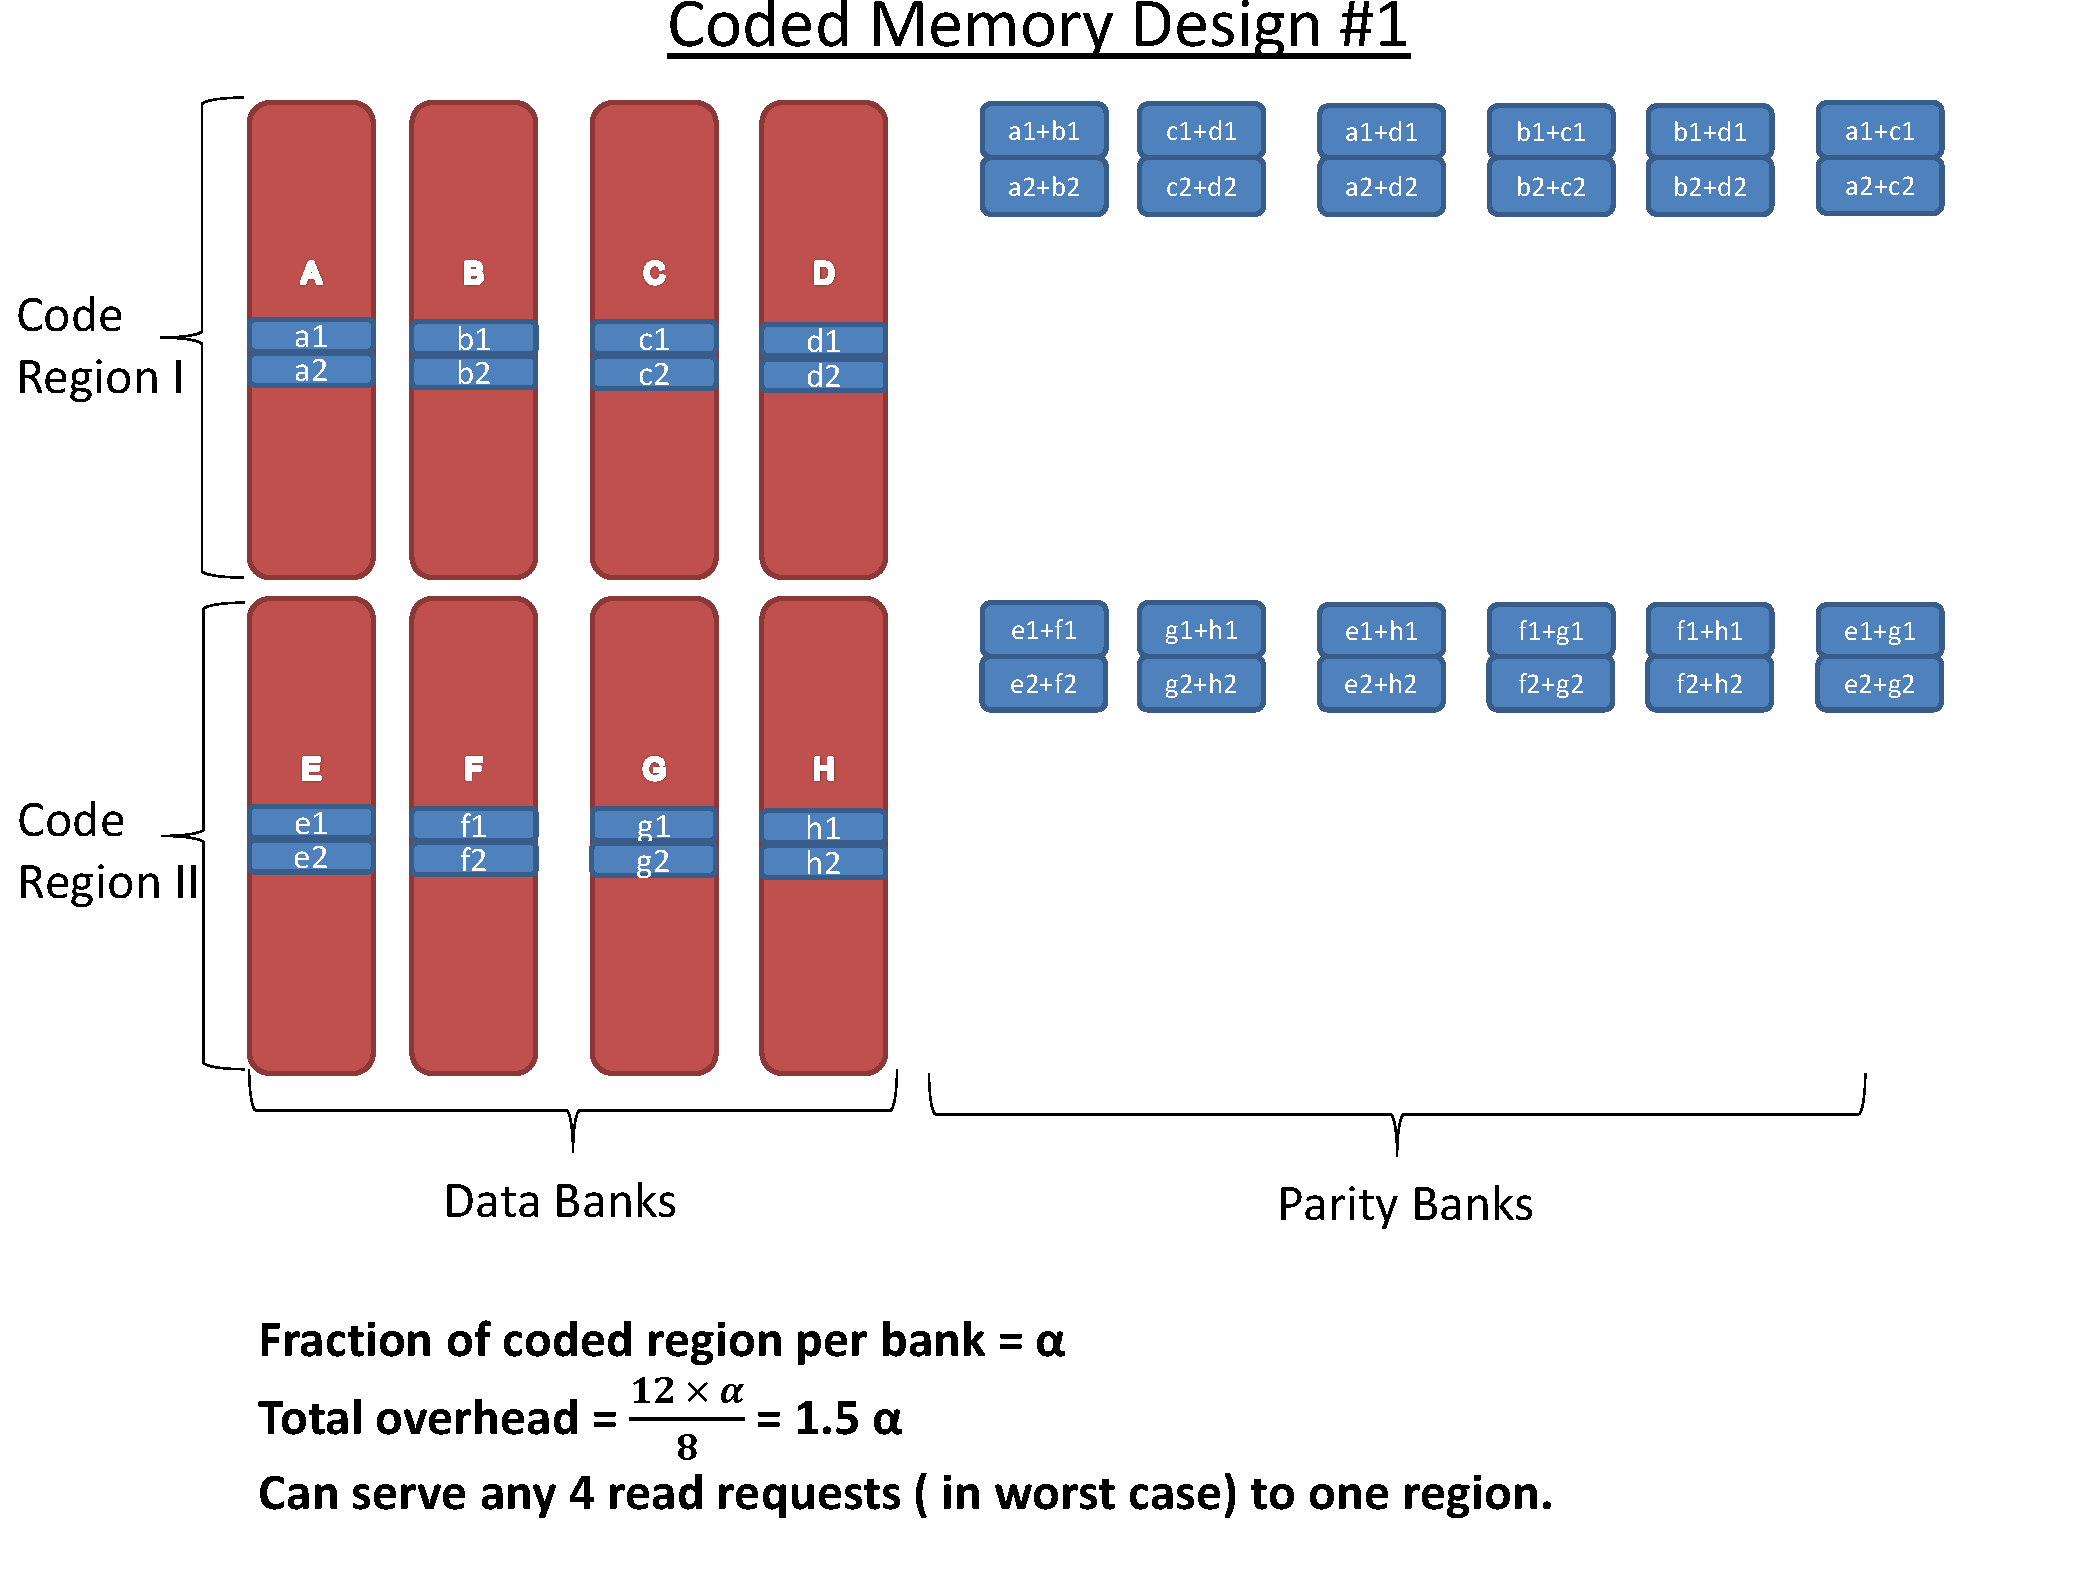
\includegraphics[width=\linewidth]{fig/designI.pdf}
	\caption{Code Design I}
	\label{fig:design1}
\end{minipage}
%\caption{Code Designs}
\end{figure} 
%------------------------------
\ignore{
%------------------------------
\begin{figure}[ht!]
\centering
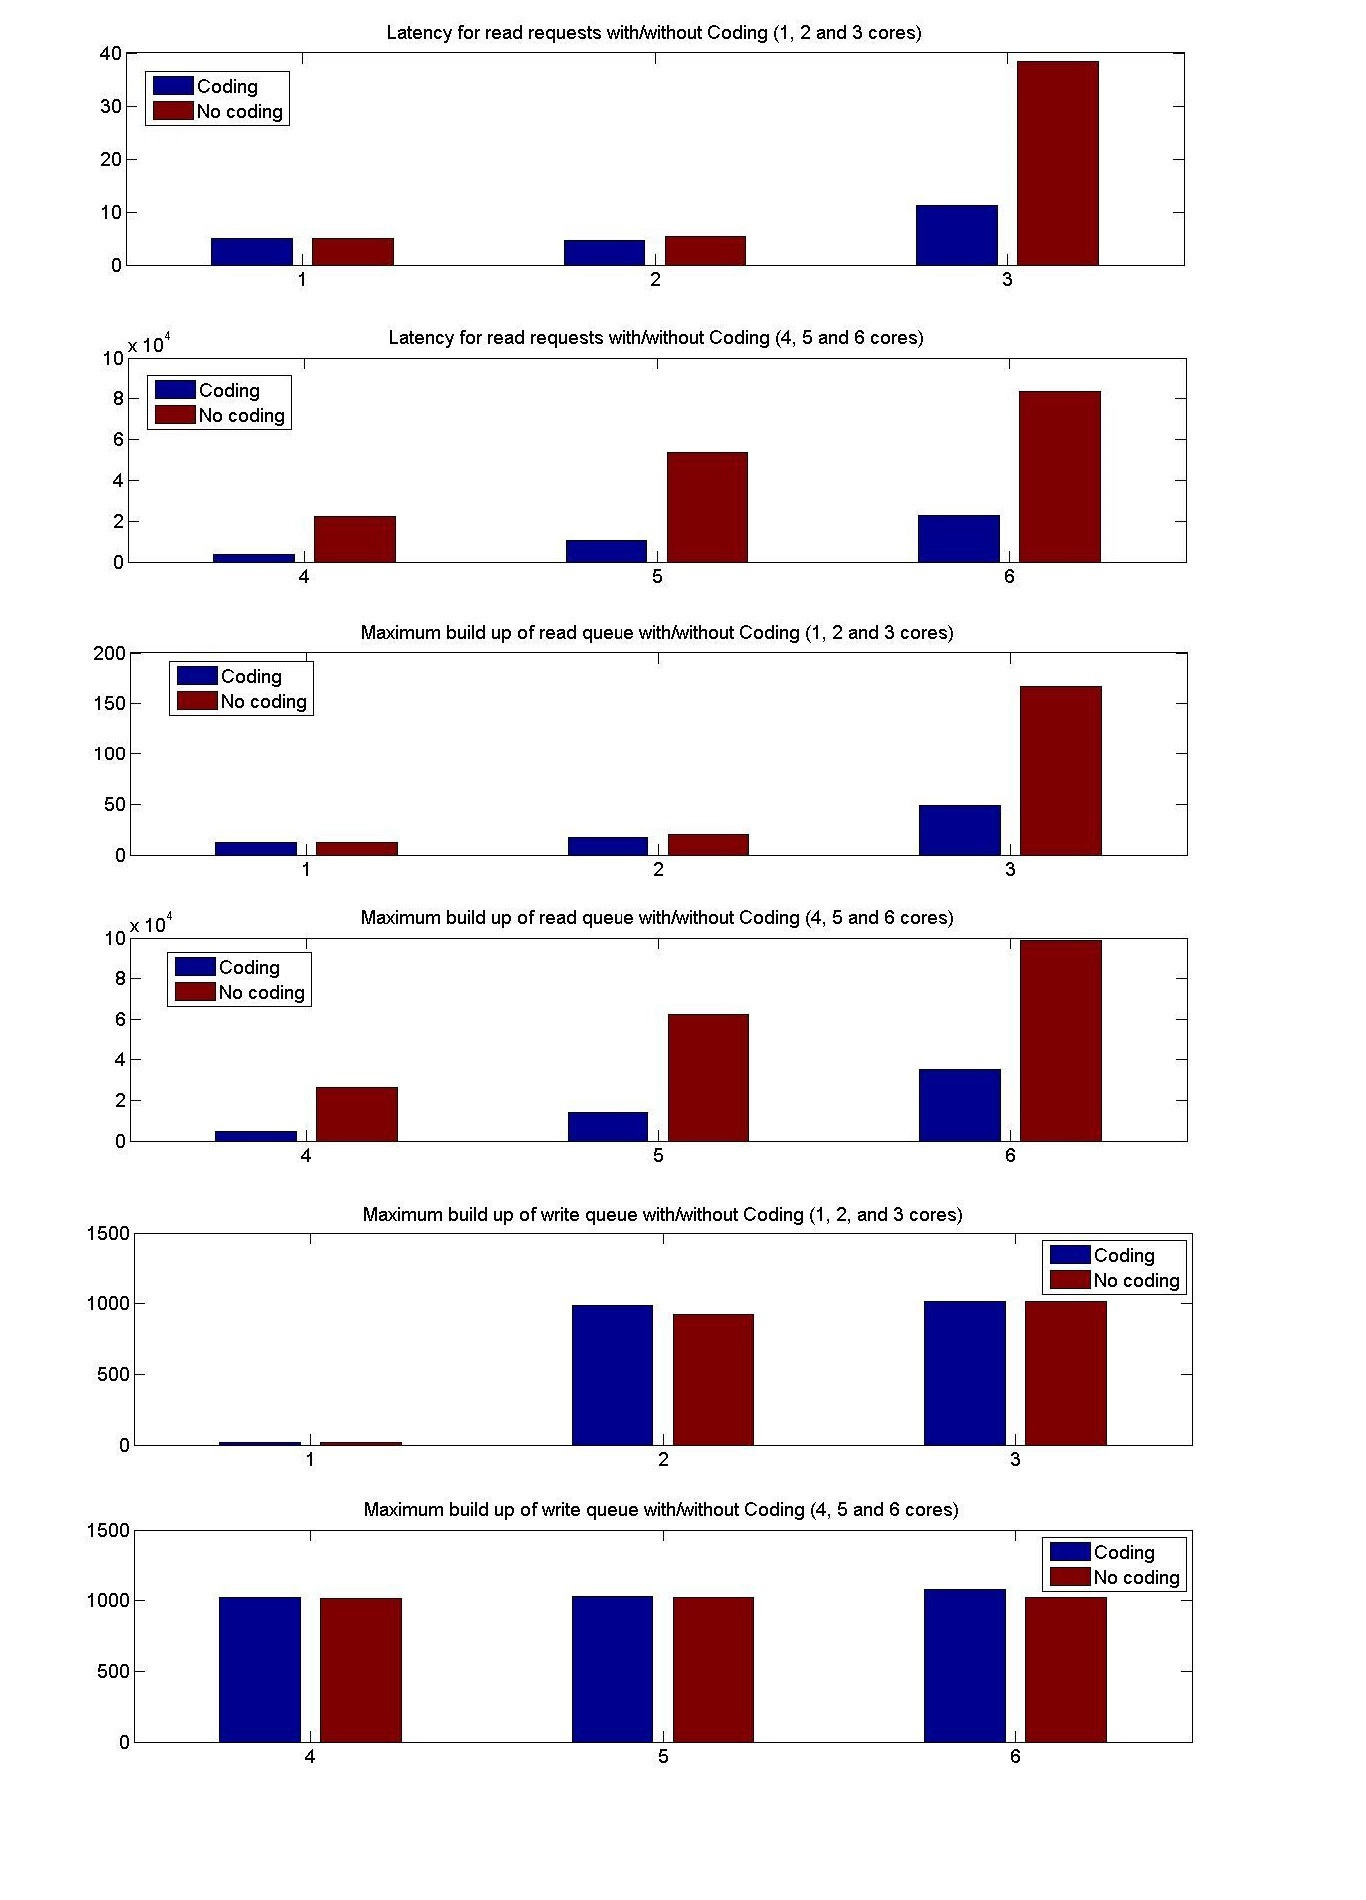
\includegraphics[width=150mm,natwidth=610,natheight=642]{fig/result_design1.jpg}
\caption{ }
\label{fig:result_design1}
\end{figure}
%------------------------------
}

\noindent \textbf{Worst case analysis}: The code design under consideration (cf.~Figure~\ref{fig:design1}) falls off to $4$ access in 
a single memory clock cycle when there are non-sequential and non-consecutive access to the memory 
banks.  For example, when the access is requested for the rows  $\{a(1), b(8), c(9), d(15)\}$. Since parity elements combining the data elements from these requested rows are not present in the parity banks, the underlying coding scheme does not provide any benefits. However, as discussed in Section~\ref{sec:prefetching}, we can use the prefetching 
mechanism to look ahead in the queue and prefetch codes from parity banks for 
the subsequent access in order to exploit the otherwise unused parity banks. 
%In Figure~\ref{fig:result_design1} , we explore the worst case scenario when 
%the accesses are random. The results show that the queue build up for reads and 
%writes does fall back to no-coding scenario. This asserts that the worst case 
%scenario for a coding scheme performs similar to no-coding scheme.In the second 
%scheme, we augment the code storage by cross storing the codes from region 1 to 
%region 2 and vice-versa.We do this in addition to coding the consecutive memory 
%addresses in a bank. This provides two benefits, first it increases the overall 
%redundancy, and second it allows us to use the parity banks of the other region 
%in case the first region�s parity banks are in use. 
Figure~\ref{fig:design2} shows the storage pattern of the codes in the bank. The 
overall overhead in this system is 2.5$\alpha$. \\
\ignore{
\begin{figure}[!ht]
\centering
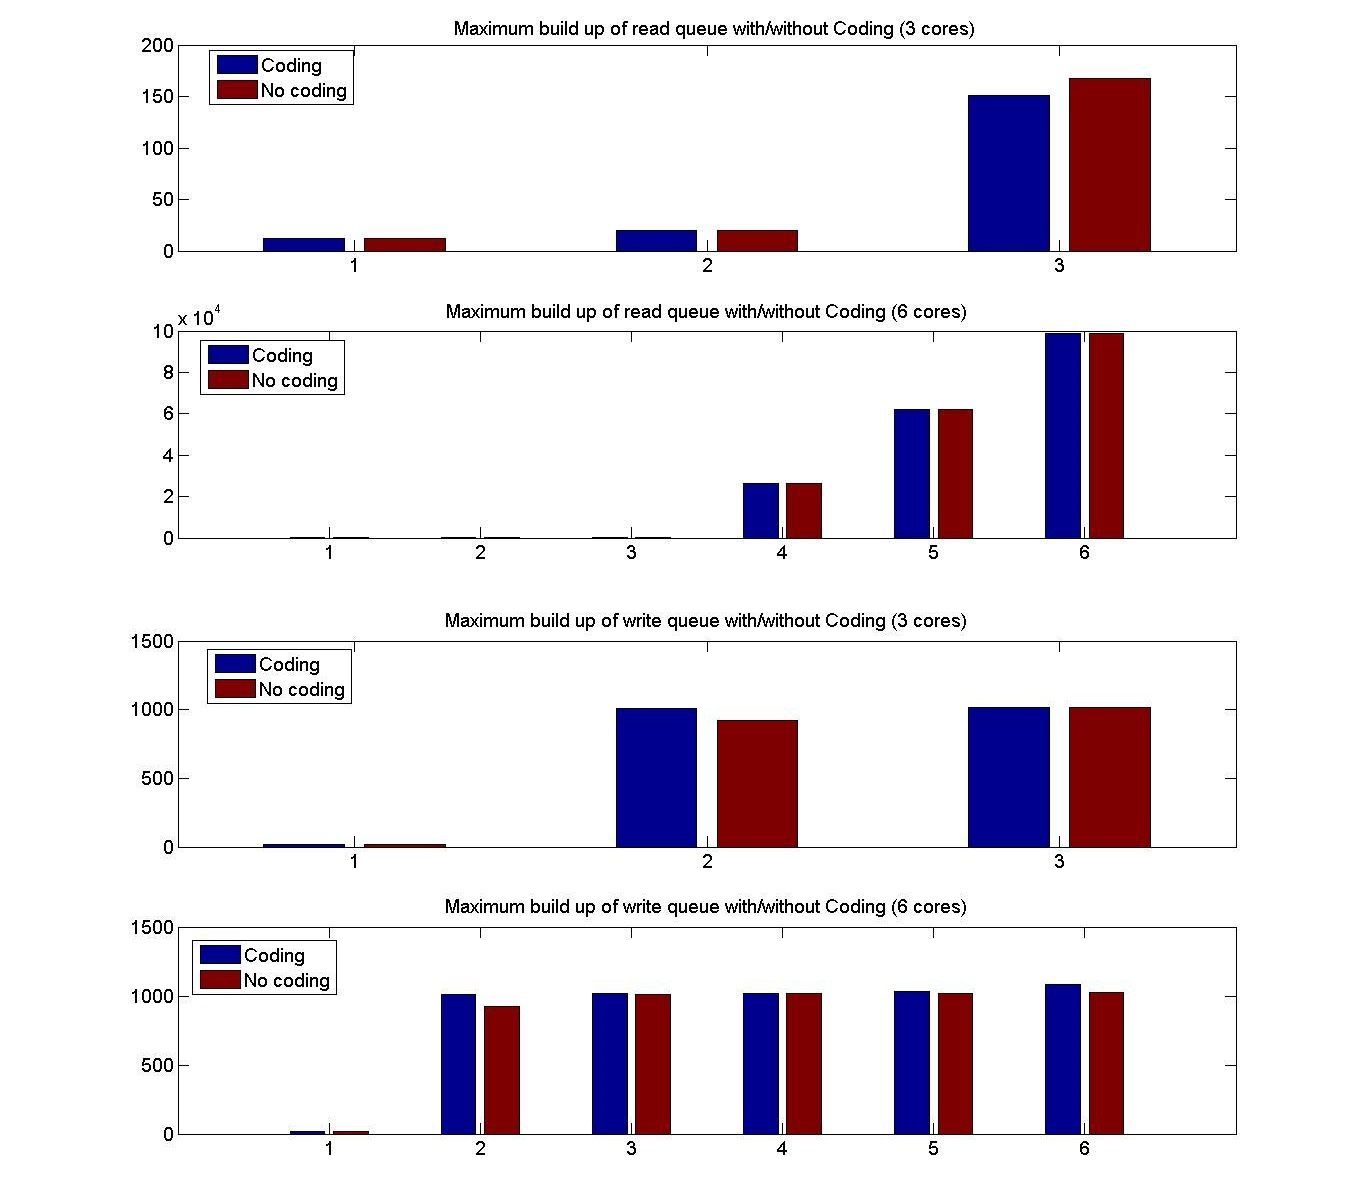
\includegraphics[width=150mm,natwidth=610,natheight=642]{fig/result_design2.jpg}
\caption{ Comparison of Design II with No coding case }
\label{fig:result_design2}
\end{figure}
}
\subsubsection{Code Design II}
The second design, presented in figure 4, improves over first design by allowing 
5 read accesses per bank per cycle. This design also divides banks into two 
regions. The first region is
Bank 1 to Bank 4 and 5 corresponding Parity banks. The two regions in figure 4 
are upper 9 banks forming one region and lower 9 banks forming another. This 
design allows intermix storage of parity among regions. The design uses 5 parity 
banks per region. The data in this scheme is coded for both inter bank and 
intra-bank. The intra-bank codes are stored in the alternate parity bank region. 
This allows usage of parity banks from other region if they are available. \\
\begin{figure}[!ht]
%\centering
%\begin{minipage}[!t]{\linewidth}
	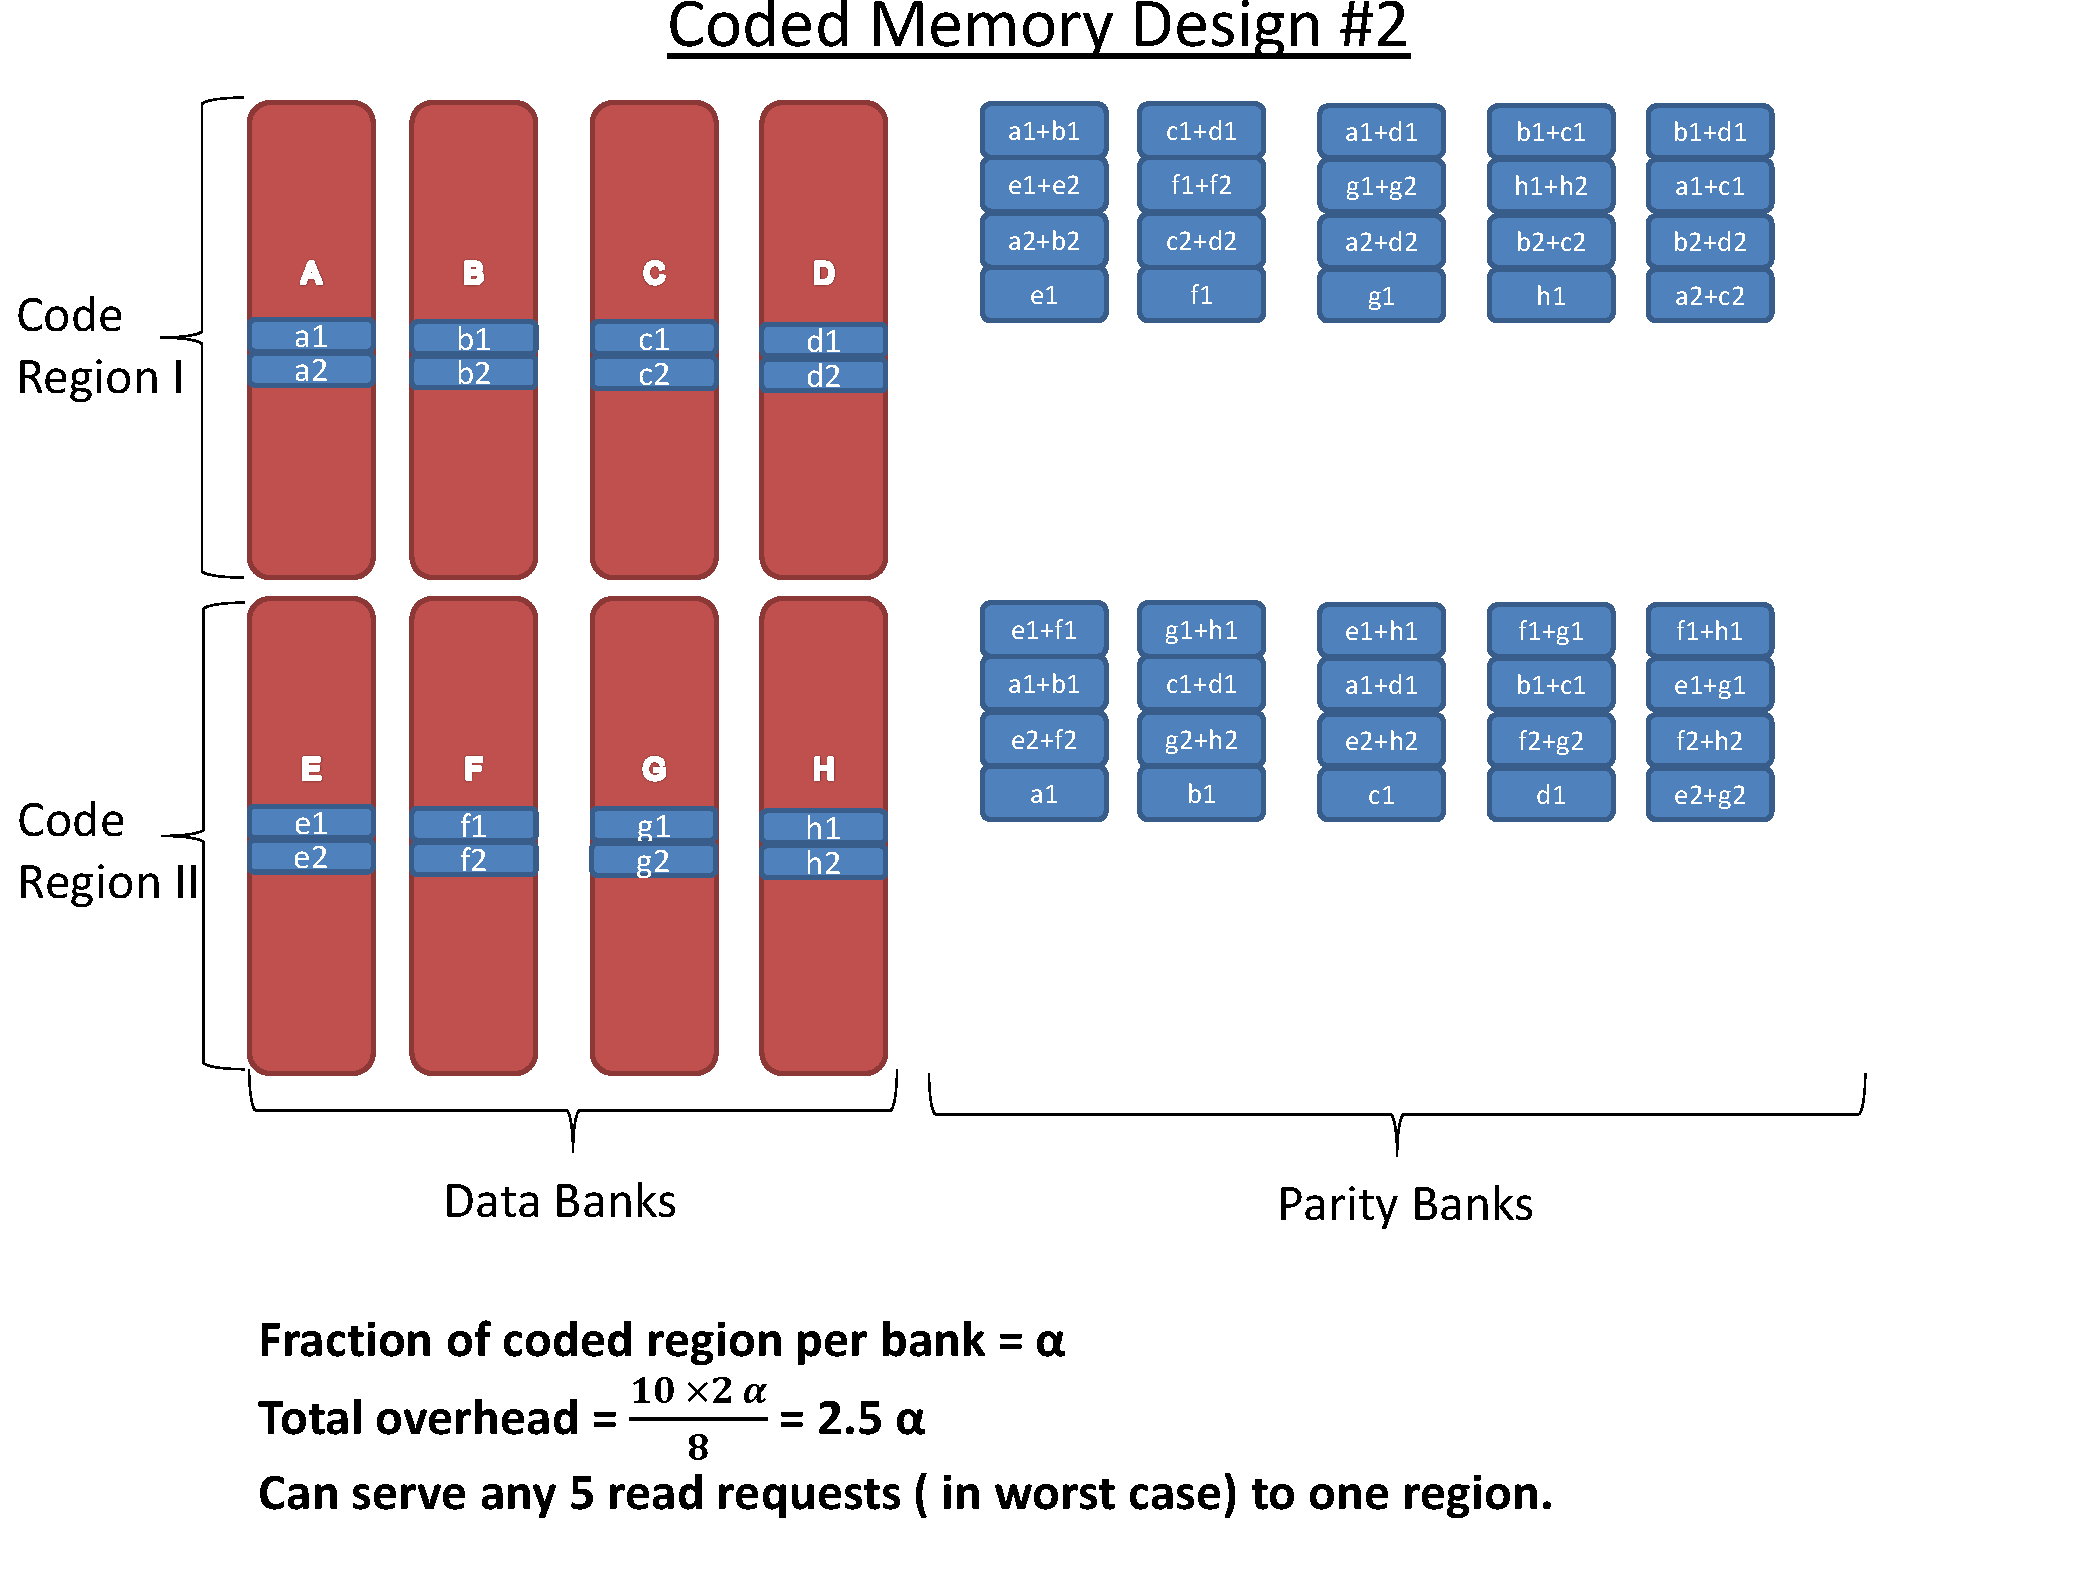
\includegraphics[width=\linewidth]{fig/designII.pdf}
	\caption{Code Design II}
	\label{fig:design2}
%\end{minipage}
\end{figure}
\textit{Best case scenario analysis}: We design this code to achieve maximum performance 
when sequential accesses to the coded regions are issued. During the best case 
access, we can achieve up to 9 parallel accesses in one cycle.
Consider the scenario if we receive accesses to 
$a_1,b_1,c_1,d_1,a_2,b_2,c_2,d_2,a_3,b_3,c_3$. Here, we can serve $a_1, b_1, 
c_1, d_1$ using $a_1$ with the parity banks $a_1+b_1,b_1+c_1,c_1+d_1$ and serve 
$a_2,b_2,d_2$ using $b_2$ with the parity banks $a_2+d_2$ and $b_2+d_2$. Lastly, 
we can serve $c_2$ and $d_3$ using bank 3 and bank 4. \\
\textit{Worst Case scenario analysis}: The code scheme can do 5 accesses in a cycle for the coded region in 
worst case.
These are non-sequential and non-consecutive accesses to the memory banks. For 
example, when the access pattern is $a_1,a_6,a_9,a_{15},a_{20}$, we can perform 
these 5 reads with the help of coded banks. We can use the prefetching 
mechanisms discussed later to look ahead in the queue and pre-fetch codes from 
parity banks for further accesses.
\subsubsection{Code Design III}
The two designs discussed above achieve a rate of $2/5$. Here, we explore a code design which achieves a rate of $1/2$. 
This design requires 9 data banks and 9 parity banks as shown in figure 5. It 
also has a comparatively higher locality of 3. That is, it requires the memory 
controller to "know" two out of three data elements to decode the third. This 
also helps us achieve 4 simultaneous read access per bank per cycle and 2 
simultaneous write access per bank per cycle. The memory overhead here is less 
(just $\alpha$) compared to the previous designs. However, it possesses higher logical complexity because of increased locality. Example cases for this design are described below :
%---------------------------------------
\begin{figure}[!ht]
	\centering
	\begin{minipage}[!t]{\linewidth}
		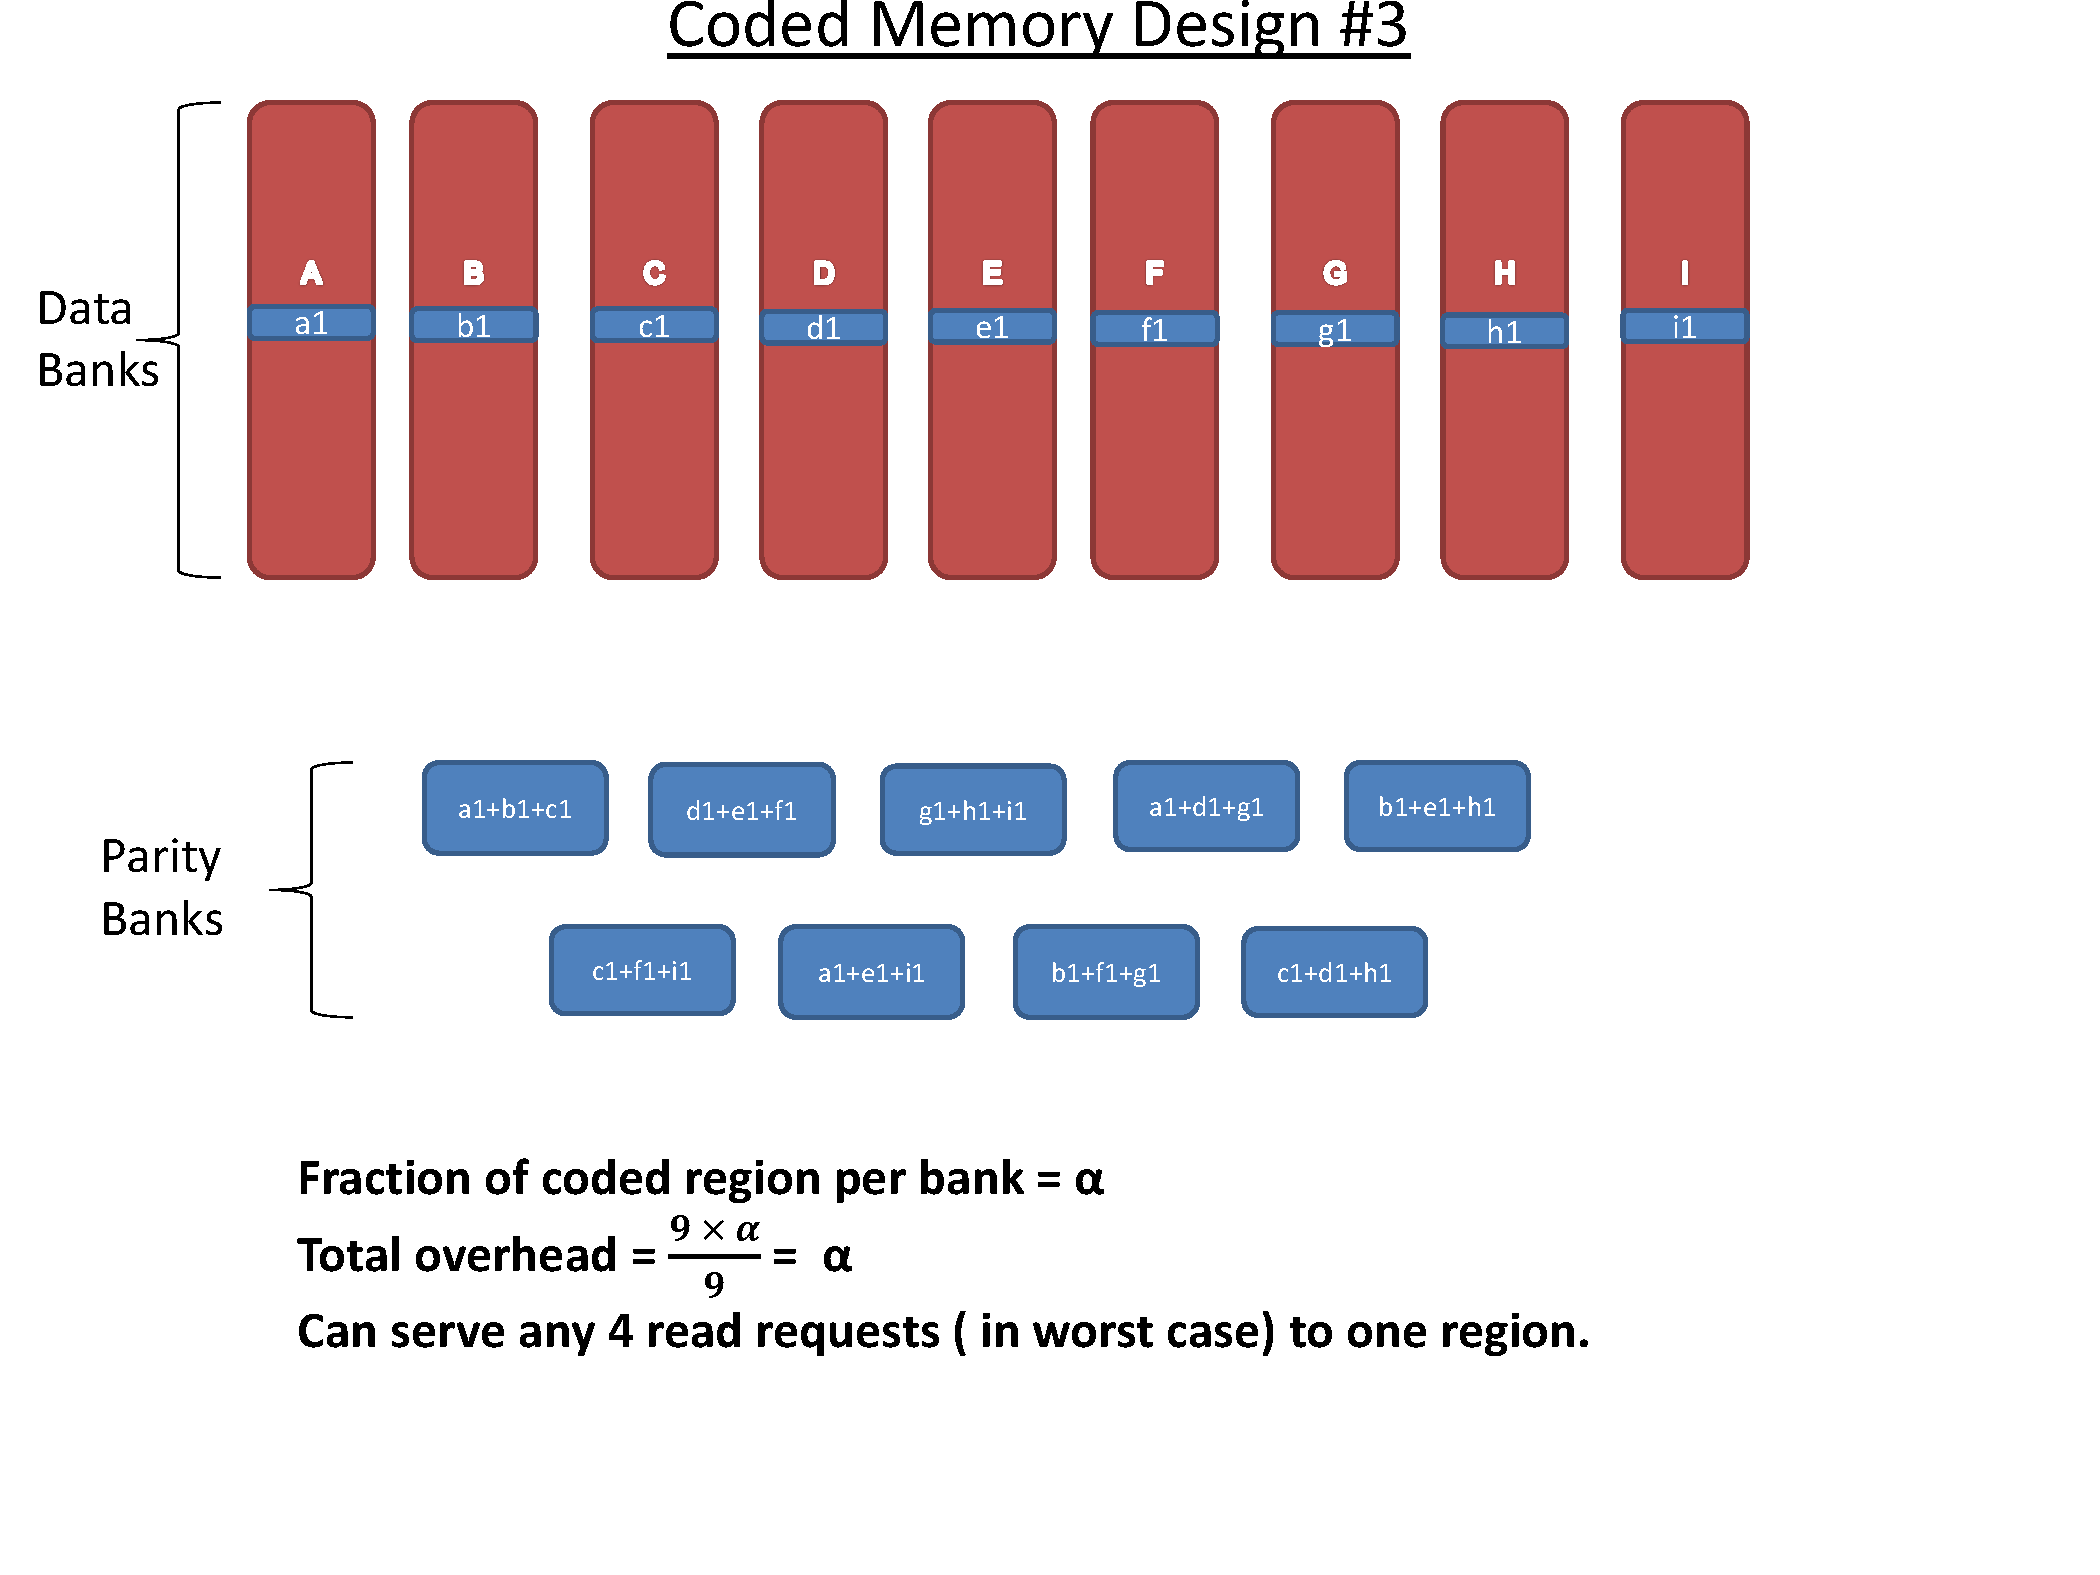
\includegraphics[width=\linewidth]{fig/designIII.pdf}
		\caption{Code Design III}
		\label{fig:design3}
	\end{minipage}
\end{figure}
%---------------------------------------
\begin{itemize}

	\item 4 reads for $a_0$: 1 read from $a_0$, 1 read from ($a_1$, $a_2$, 
		$a_0$ + $a_1$ + $a_2$), 1 read from ($a_3$, $a_6$, $a_0$ + $a_3$ 
		+ $a_6$), and the 4th read from ($a_4$, $a_8$, $a_0$ + $a_4$ + 
		$a_8$).
	\item 3 reads for $a_0$: 1 read from $a_0$, 1 read from ($a_3$, $a_6$, 
		$a_0$ + $a_3$ + $a_6$), and the 3rd read from ($a_4$, $a_8$, 
		$a_0$ + $a_4$ + $a_8$). \\
	      1 read for $a_1$:  1 read from $a_1$.
	\item 2 reads for $a_0$: 1 read from $a_0$ and the 2nd read from ($a_3$, 
		$a_6$, $a_0$ + $a_3$ + $a_6$). \\
	      2 reads for $a_1$: 1 read from $a_1$ and the 2nd read from ($a_4$, 
	      $a_7$, $a_1$ + $a_4$ + $a_7$).
	\item 2 reads for $a_0$: 1 read from $a_0$ and the 2nd read from ($a_3$, 
		$a_6$, $a_0$ + $a_3$ + $a_6$). \\
	      1 read for $a_1$: 1 read from $a_1$. \\
	      1 read for $a_2$: 1 read from $a_2$.
    \end{itemize}
Figure~\ref{fig:design3} describes the system with 9 data banks and 9 parity bank. 
Since most systems are implemented with number of banks as $2^n$ for some n. We present an 
example of the code with 8 data banks in figure~\ref{fig:design3_8}. For using 8 data banks, 
we drop the bank I. We also ignore the data from Bank I for constructing parity. So, three of 
the parity banks have the locality of 2, while the rest of the parity banks have locality of 3.
 The new scheme for 8 data banks has 9 parity banks.
%---------------------------------------
\begin{figure}[!ht]
\centering
	\begin{minipage}[!t]{\linewidth}
		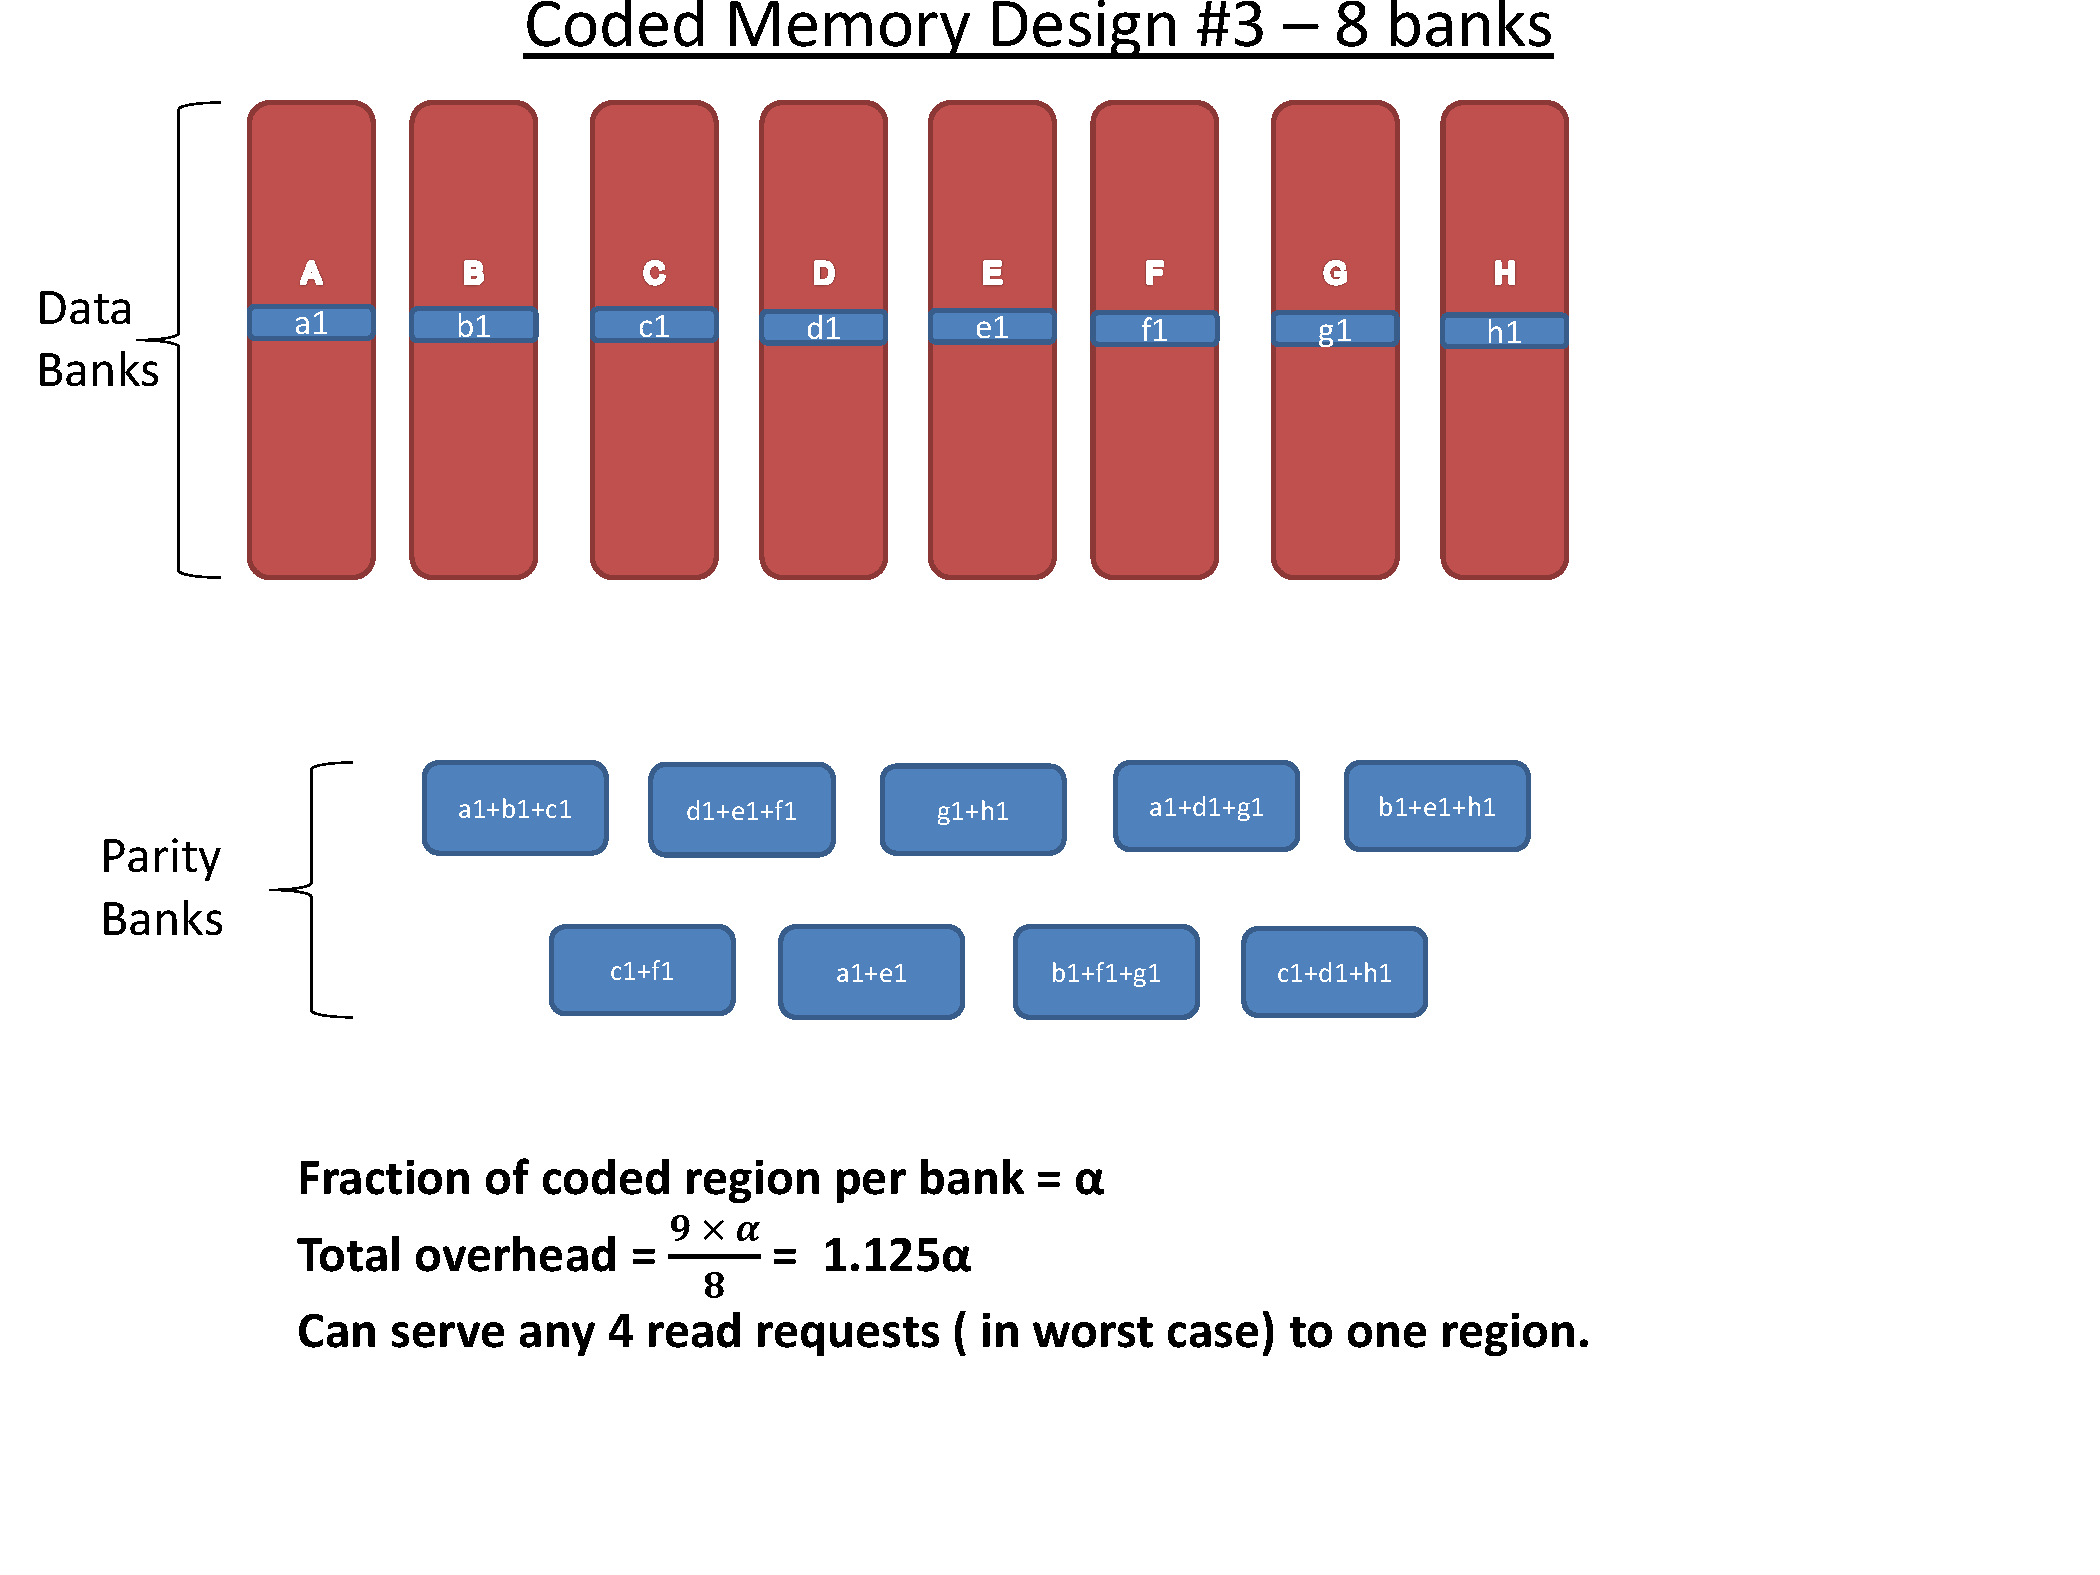
\includegraphics[width=\linewidth]{fig/designIII_8banks.pdf}
		\caption{Code Design III with 8 data banks}
		\label{fig:design3_8}
	\end{minipage}
\end{figure}
%---------------------------------------
Since the locality is 3 here in this design, i.e. , each parity is made up of combination of 3 data banks, we need to make sure that all three requests are in one line to be able to use the parity bank. 
For example parity bank 0 contains A+B+C. So, the following scenarios arise:
\begin{itemize}
	\item {\em Scenario I}: 1st request of A and 1st request of B are in same row. Then, we can search for a request in the same row for bank C by doing a look ahead. 
	\item {\em Scenario II}: 1st request of A and 1st request of C are in same row. Then, we can search for a request in the same row for bank B by doing a look ahead. 
	\item {\em Scenario III}: 1st request of B and 1st request of C are in same row. Then, we can search for a request in the same row for bank A by doing a look ahead. 
\end{itemize}
So, the simple pseudo code for doing this would be :\\
\begin{verbatim}
for each data bank 
    for each auxiliary bank1 of data bank
            Look ahead in auxiliary bank2 and check if 3 request in a row.
        end
    end
\end{verbatim}
Example: - \\
For {\bf data bank} to be {\bf A} \\
{\bf auxiliary bank1} goes from [B C D G A E] \\
{\bf auxiliary bank2} goes from [C B G D E A] \\
  The element A is just there in {\bf auxiliary bank1} and {\bf auxiliary bank2} to maintain the symmetry because A + E has locality of 2.

